

%-----------------------------------------------------------------------------
% SK Detector Systematics
%-----------------------------------------------------------------------------
\section{SK Detector Systematics for fiTQun Selection}
\label{sec:skerr}

With the fiTQun topological selections specified in TN-319~\cite{tn319} and the FV cuts
for each selection specified in Section~\ref{subsec:fvresults}, all of the necessary
cuts for T2K event samples have been defined.  In this section, we address the
problem of estimating the detector systematic uncertainties for each sample.
The overall procedure here follows closely that of previous analyses such
as TN-186 and the toy MC studies of Section~\ref{subsec:fvunc}.  First, the
results of the atmospheric fit are applied to the T2K
event selections using toy MC studies. The result of this study is a covariance
matrix of the uncertainties for various MC event categories and in various
visible energy regions.  This covariance matrix is then used as an input to
another toy MC study that adds contributions from additional uncertainties to
produce the final SK detector errors for the fiTQun samples.  This section will
focus on the initial covariance matrix generated from the atmospheric neutrino
fit described in Section~\ref{sec:fitresults}.  Details of how the final SK
detector systematics are calculated can be found in TN-317~\cite{tn317}.

To generate the detector uncertainties from the atmospheric neutrino fit, we
perform a toy MC study were we once again draw samples from the post-fit Markov
chain and apply them to various selected MC categories.  The categories are
taken from TN-186 and are defined in Table~\ref{tab:errcat}. The quantity to
be estimated for each event category is the fractional efficiency of the ``core''
cuts applied after the ``base'' cuts.  For this analysis, we choose to remove the 
dependence on the atmospheric flux and cross section, and normalization parameters by 
marginalizing over them.  The fractional change in efficiency then depends only
on the distribution shape parameters $\beta$ and is calculated from:
%
\begin{equation}
  \label{eq:deleff}
  \Delta \varepsilon(\beta) = \left[ \frac{1}{\varepsilon_{0}}
  \int\int\frac{N_{core}(\alpha,\gamma,\beta)}{N_{base}(\alpha,\gamma)}d\alpha d\gamma \right] - 1
\end{equation}
%
where $\varepsilon_{0}$ is the nominal efficiency from the MC.

The procedure for calculating the uncertainty of $\Delta \varepsilon$ is nearly
identical to the procedure used to estimate the detector systematics in the various
detector regions described in Section~\ref{subsec:fvunc}. The steps are outlined
below:

\begin{enumerate}
  \item Choose a random sample set of fit parameters from posterior Markov chain.
  \item Loop over the atmospheric neutrino MC events, and for each event directly modify the fiTQun cut variables
    according to Equation\ref{eq:fqparmod}. Also apply normalization factors according the drawn $\alpha$ and
    $\beta$ parameters.  Then apply the ``core'' cuts defined in Table~\ref{tab:errcat}.
  \item Calculate the marginalized efficiency from Equation~\ref{eq:deleff} (requires an additional
    loop varying only $\alpha$ and $\gamma$ parameters).
  \item Repeat from Step 1 until a suitable number of toy samples have been generated
  \item Calculate the variance and covariance over the toy experiments for each category defined
    int Table~\ref{tab:errcat} and in various visible energy bins.
\end{enumerate}

The correlation matrix obtained by through executing this procedure can be seen
in Figure~\ref{fig:skcorr}.  Strong correlations are present between the
visible energy bins of each category.  This comes from the detector error
parameters not having an explicit visible energy dependence, which results in
each visible energy bin receiving the same set of $\beta$ parameters.  The
efficiency uncertainty for the \nue samples comes almost entirely from the
variations of the fiTQun $\pi^{0}$ likelihood distribution when the $\beta$
parameters are applied.  Since the $\pi^{0}$ cut is not applied to the \numu
samples, the \numu uncertainties are much smaller and come from the variations
in the fiTQun $e/\mu$, $\mu/\pi$, and $1R/2R$ likelihoods.  The overall
uncertainties for each category are shown in Figure~\ref{fig:skunc}.

\begin{table}
  \centering
  \begin{tabular}{l | l | l}
    \hline\hline
    Category & Base Cuts & Core Cuts \\
    \hline
    \nue CC1e & 1 electron ring, $N_{decay} = 0$, $p_{e} > 100$ MeV & e-like, not $\pi^{0}$-like, 1R-like \\
    \nue CC Other & electron + other rings, $N_{decay} \ge 1$, $p_{e} > 100$ MeV & e-like, not $\pi^{0}$-like, 1R-like \\
    \numu CC1$\mu$ & 1 muon ring, $N_{decay} = 1$, $p_{e} > 30$ MeV & $\mu$-like, not $\pi$-like, 1R-like \\
    \numu CC Other & muon + other rings, $N_{decay} \ge 2$, $p_{e} > 30$ MeV & $\mu$-like, not $\pi$-like, 1R-like \\
    \hline
  \end{tabular}
  \caption{Definitions of the MC event categories for the detector error covariance matrix.}
  \label{tab:errcat}
\end{table}

\begin{figure}[ht]
  \begin{center}
    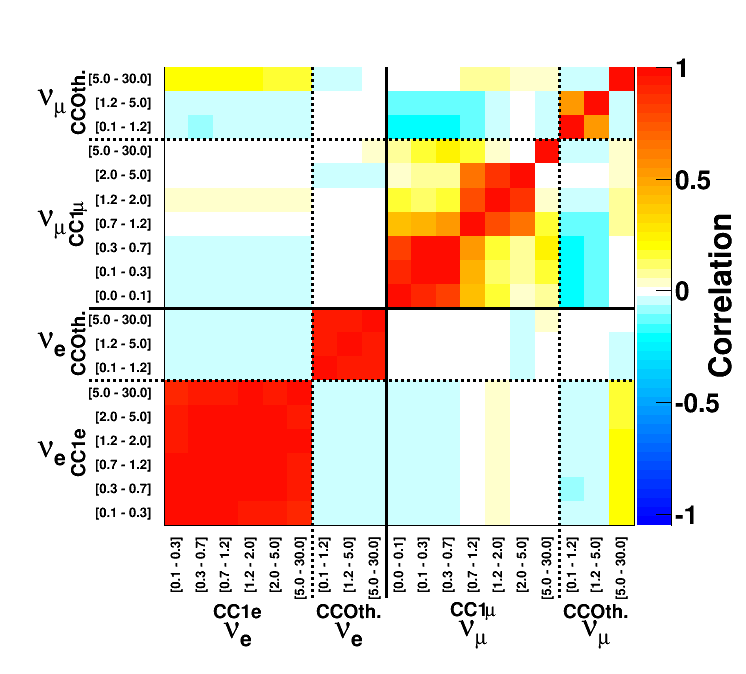
\includegraphics[width=0.65\textwidth]{hcor_v2}
  \end{center}
  \caption{Correlation matrix for the efficiencies of the core cuts for
  various MC categories in various visible energy regions.}
  \label{fig:skcorr}
\end{figure}

\begin{figure}[ht]
  \begin{center}
    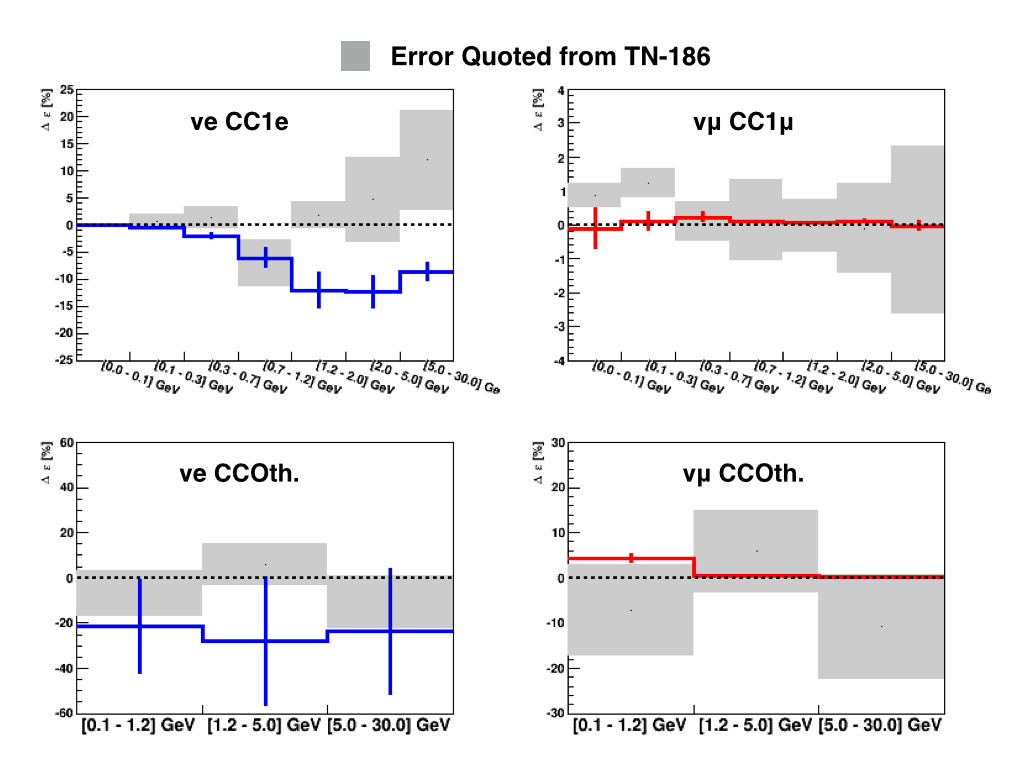
\includegraphics[width=0.5\textwidth]{skerrs_1D}
  \end{center}
  \caption{Detector systematics for each of the MC categories defined in Table~\ref{tab:errcat} and 
  in various visible energy bins.}
  \label{fig:skunc}
\end{figure}










